\section{Introduction}
\label{sec:introduction}

Location information is becoming increasingly popular in online social networks, vehicle networks, and online games. Companies like Google and Uber have heavily invested in autonomous vehicles that make driving decisions based on real-time highly accurate location coordinates~\cite{markoff2010google}. On smartphones, more users are sharing location data through multiple types of apps, ranging from navigation maps to geographically enhanced games, such as the hugely popular game Pokemon Go~\cite{pokeman}. In these scenarios, one big concern has been the privacy of users, as unexpected leaks of users' location trajectories will allow potentially malicious attacks to gain advantages in the real-world~\cite{locationprivacy}. For example, by knowing when a user leaves and returns home each day, a potential third-party attacker could identify the time periods during which the user’s home is not occupied.  The attacks range from mild inconveniences such as privacy leaks to much more serious attacks such as break-ins, among other types of attacks.

One significant challenge on keeping location data secure is that we should not trust servers as safe against attacks~\cite{krutz2010cloud}. Indeed, the significant increase on hacking activities against servers in recent years~\cite{liao2013intrusion,grispos2013calm} means that if we store non-encrypted data on servers, we will face the risks that such data may be leaked when the severs themselves compromised. Perhaps paradoxically, when building apps that involve location data, servers typically perform extensive computation on the location traces, making it necessary for the servers to be able to decrypt data as needed. For example, Google Maps needs to obtain the starting and ending locations to calculate the trajectories for navigation purposes, and Facebook servers need users' geographic regions to accurately deliver targeted advertisements. So the challenge is, is it still possible for us to maintain security of location traces while \emph{allowing} servers to perform app-specific computations?

Given the demands from users to keep their location data secure, as well as the need for the servers to perform basic operations on the trajectory data, in this paper, we investigate methods such that we can achieve both goals simultaneously. Specifically, we develop secure computation primitives on location data where the servers should have no knowledge on the plaintext, i.e., the servers should not even keep the private keys to decrypt data. In this way, compromised servers will not cause leaked user data. Our work is motivated and enabled by the recently developed homomorphic computing principles: recent advances in this area has demonstrated it is feasible to perform meaningful and predictable computations on encrypted data without decrypting them first~\cite{Gentry:2009:FHE:1536414.1536440,ahn2015computing}. In our work, we build on these homomorphic principles, and focus on one commonly used primitive in location data processing: computing the intersections between location datasets. Such a primitive can be used for many apps, ranging from deciding if users' trajectories match query requirements for targeted advertisement deliveries, to suggesting the most appropriate users for ride-sharing purposes.

Specifically, our computational primitive works as follows: we consider two users, Alice and Bob, to find out if their location datasets (e.g., such sets could be collections of singleton locations, or continuous trajectories, or areas within specified boundaries) have intersections. The application model is as follows: Alice can publish her location dataset after encrypting them first, via an aggregation server (e.g., her Facebook page), meaning that Bob does not get access to the data directly. Instead, Bob can send a query to the aggregation server by using his location sets as the query key. Note that as Bob also cares about his privacy, Alice should not see the plaintext of Bob’s location set neither. Hence, Bob should avoid sending plaintext in the query. Next, the aggregation server performs the \emph{matching} step, where Alice's secured datasets are matched against Bob's query, and a (still encrypted) computational result is returned to Alice. Alice can decide whether there is an intersection between the incoming query and her datasets by decrypting the result using her own private key. If there is an intersection, Alice is able to send additional information to Bob, possibly through the help of the aggregation server since it knows Bob's identity (e.g., social media accounts or emails).

We now make a few remarks on this computational model. First, by design, this model ensures that the location datasets are fully secure, as Alice will only publish the datasets that are encrypted using her public key. On the side of Bob, as we will explain later, the plain text is also processed using hash functions. By choosing sufficiently strong cryptographic hashing functions, we can also ensure that the plain text of Bob is well protected. Hence, Alice and Bob do not directly share the plaintext of their location histories. Second, this computational model is sufficiently secure against compromised servers, as the aggregation server does not keep any plaintext of location trajectories. Finally, only queries that return positive results (i.e., there are intersections) will lead to further interactions between Alice and Bob.

The central methodology in our implementation is based on an advanced data structure called the bloom filter, which has been widely adopted in the networking literature~\cite{broder2004network}. Our work, to our knowledge, is the first to propose a homomorphic version of this data structure. In our design, we offer both a standard form design as well as two optimized designs, and compare their performance. Figure~\ref{fig:architecture} shows an overview of the proposed framework, where the actions taken by Alice, Bob, and the aggregation server are illustrated. 

\begin{figure}[t]
	\centering
	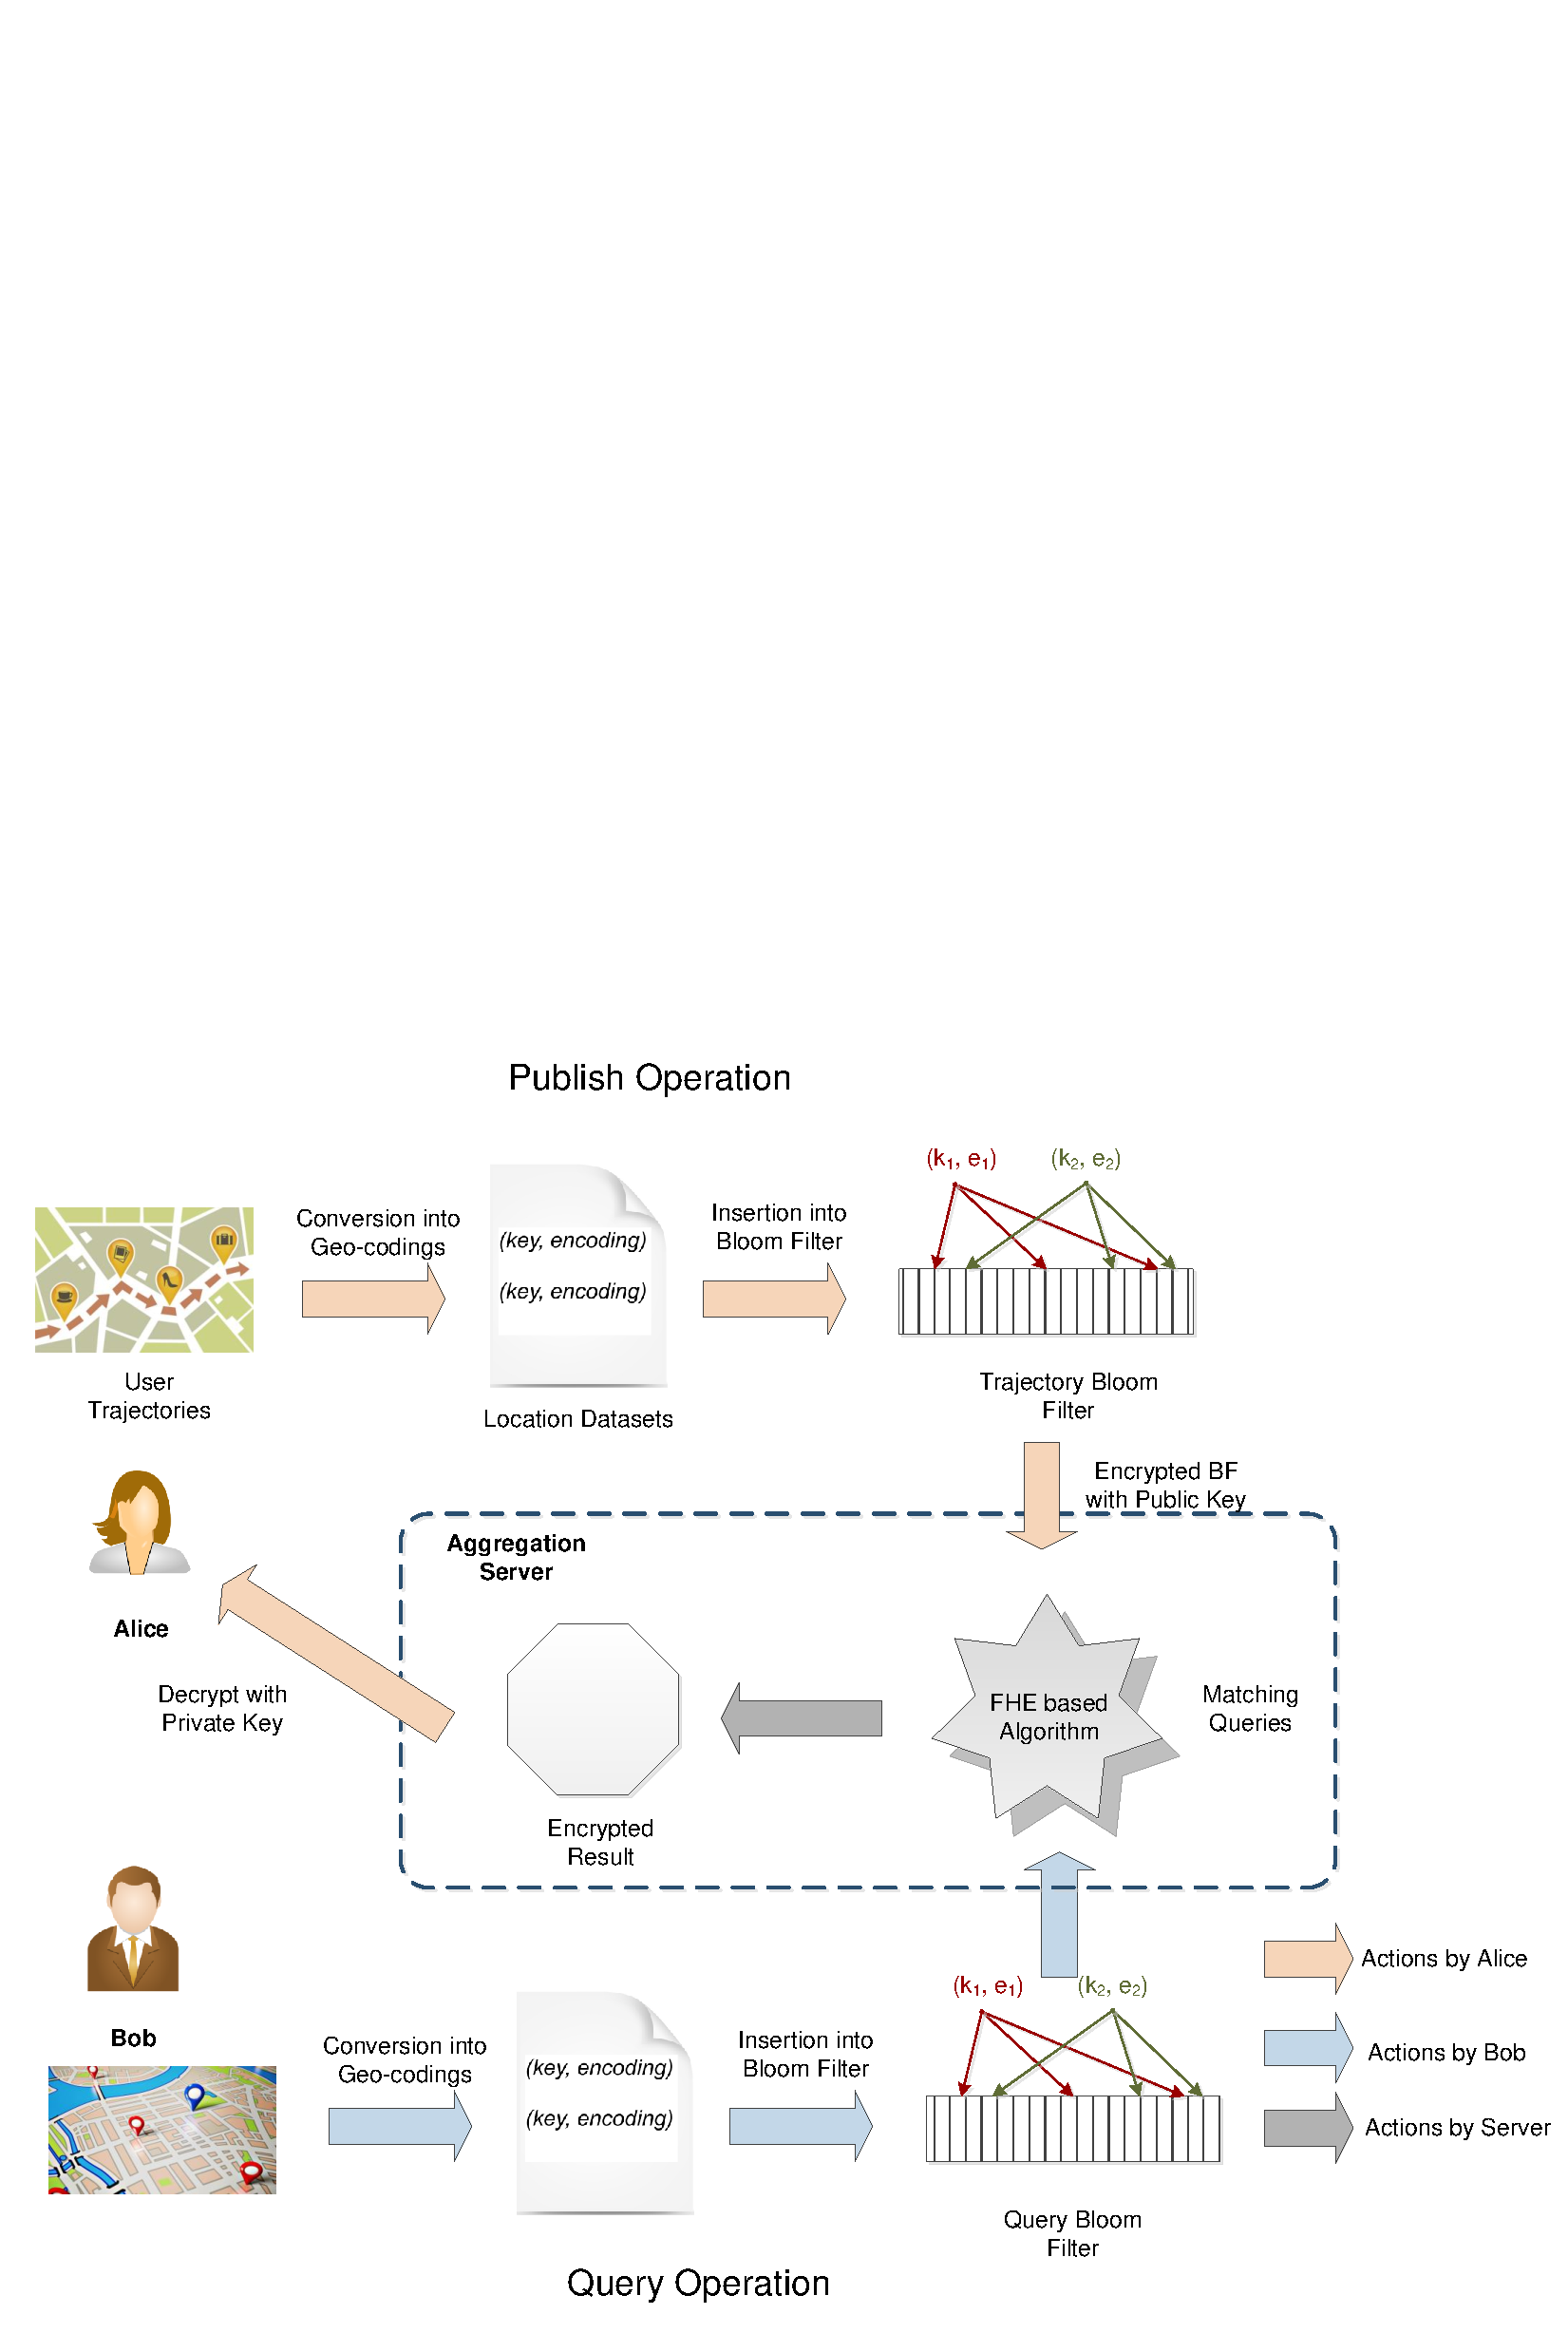
\includegraphics[width=0.8\linewidth]{figures/architecture.pdf}
	%\vspace{-0.1in}
	\caption{Computational model architecture}
	\label{fig:architecture}
	\vspace{-0.1in}
\end{figure}


Another major contribution of this paper is that we develop a distributed protocol that allows one party to determine, in a private and secure manner, whether or not a second party's trajectory has an intersection with the first party. Our design is fully flexible, meaning that each user is able to specify what kind of datasets they would like to make visible, and be queried by other users. The location datasets can include trajectories, areas, and isolated points. For areas, we also present a geohash based optimization that allows areas to be represented in a compact and flexible manner. 

The third contribution this paper is that we offer a working prototype, which is implemented on the open-source homomorphic libraries. Our preliminary results demonstrate the feasibility of the proposed approach as well as the security of the protocol designs. We also evaluate the performance of our implementation with a real-world dataset that is collected in a city area on users' smartphones to demonstrate the effectiveness of large-scale location queries.

The remaining of this paper is organized as follows. In Section 2, we describe the related work to our paper. In Section 3, we describe the problem formulation and the protocol design. In Section 4, we describe the prototype design and implementation details. In Section 5, we describe the analysis of security. In Section 6, we describe the evaluation results. In Section 7, we describe the conclusions.
